\chapter{Background of Trans-Himalayan languages}\label{c:THOverview}

\section{Introduction}
The \lfam\ family, also referred to as Tibeto-Burman or Sino-Tibetan\footnote{The term `Tibeto-Burman' is used in the literature to refer to both the family as a whole, as well as a single branch. This is discussed in full in \sref{ss:THOverview:Name}.}, is a primary language family spoken throughout parts of Asia, centring on the Himalayas and extending to the south-east through Myanmar and the Shan Hills, to the north through to the northern edge of the Tibetan Plateau, and to the west into the Karakoram mountains and Baltistan. Languages of this family are also spoken throughout China, both historically and as the official language of China, namely Standard Mandarin (\textit{pǔtōnghuà}). Their overall geographic distribution is shown in \mapref{fig:OverallMap}, showing the family stretching as far north as Northern China (Mandarin, Sinitic), to the western reaches of the Himalayan range in Kashmir in the west (Purik and Balti, Tibetic). In the south, the Karen subfamily stretches south towards the Malay Peninsula; in the east, more recent migrations have brought Sinitic Languages to Taiwan. The family includes major languages such as Mandarin and Cantonese, both in the Sinitic branch; Burmese, in the Ngwi-Burmese branch; and Tibetan, in the Bodish or Tibetic branch. Additionally, some smaller languages have official status or institutional support such as Dzongkha and Denjongke (Tibetic) in Bhutan and Sikkim respectively. The remainder of the languages in the family are, for the most part, spoken by smaller indigenous communities throughout the region. Glottolog reports almost 500 languages in the family \cite{glottolog}, while \citeA{Owen-SmithHill2013} report around 600, with over 1.4 billion total speakers \cite{ZhangH2020Baye}, approximately 900 million of which are native Mandarin speakers \cite{Ethnologue}. While the majority of the family's speakers exist to the North of the Himalayan range in China, this statistic is a result of the overwhelmingly large number of speakers of Sinitic languages, specifically Mandarin and its dialects. The greatest area of linguistic diversity, on the other hand, falls to the South, in the Eastern Himalaya region covering Eastern Nepal and far North-Eastern India, in particular in the Shan Hills \cite{BlenchPost2014}.

This chapter comprises an overview of the history of research into the \lfam\ family in Section \ref{s:historyofresearch}, both in the Western tradition and otherwise, a major part of which is the growing body of grammatical description that provides a foundation for this project. It also provides an overview of some ongoing contemporary discussions and research in the field in Section \ref{s:THOverview:CurrentResearch}, and establishes the stance taken in this project with regards to these disagreements. Within this, Section \ref{ss:Methods:Bayesian} compares a number of proposed phylogenies, in particular those developed through Bayesian analyses in \citesA{Sagart2019Baye}{ZhangM2019Baye}{ZhangH2020Baye} and discusses some potential issues with the conclusions they draw. It will also consider the usefulness of these methodologies and their results both in the development of a representative sample and in linguistics in general. Lastly, this chapter discusses the work that has been undertaken in the historical domain, looking both at surviving primary sources of historical languages, as well as the current extent of reconstructions of proto-languages.

\begin{map}
\centering
\includegraphics[width=\textwidth]{FullExtent.png}
\caption{The approximate full extent of the \lfam\ languages, missing some parts of the People's Republic of China, and of Taiwan. There are areas inside this extent where \lfam\ languages are not spoken, or where non-Trans-Himalayan languages are spoken (e.g. Kra-Dai, Austroasiatic, Mon-Khmer, Indo-European).}
\label{fig:OverallMap}
\end{map}


\section{History of research into \lfam\ languages}\label{s:historyofresearch}
\subsection{Pre-European scholarship}
Linguistic research is no new innovation in the Himalayas and Eastern Asia. Scholars wrote about language and its history and use well before the arrival of any Western academic tradition to the region. Literary traditions have existed in a number of regions for many centuries, and much of this literature informs contemporary linguistic research.

Old and Middle Chinese Rime Books, which group characters by their pronunciations, have been widely used as sources informing contemporary reconstructions of the languages \cite{Baxter1992}. The books were composed as early as the second century CE, through to the ninth. Due to the (generally) non-phonetic nature of the Chinese writing system, these books were compiled to create some record or method of instruction into the pronunciation of each character, by sorting each character in terms of its onset and rime \cite{Ji2021}.

There is a similarly longstanding tradition of linguistic research in Tibet. Perhaps the most important of these are the \texttibetan{སུམ་ཅུ་པ} \textit{Sum cu pa} and \texttibetan{རྟགས་ཀྱི་འཇུག་པ} \textit{rTags kyi 'jug pa}, both attributed to 7th century scholar Thönmi Sambhoṭa, who is also credited with the development of the Tibetan writing system \cite{MuellerWitter2009}. These treatises comprise early grammatical descriptions of the language at the time, and are, at least according to legend, the only two survivors of a corpus of eight written by Thönmi Sambhoṭa \cite{Miller1963}. They are also accompanied by a tradition of more recent of commentaries and translations \cite{Chashab2008}. There have been questions raised as to whether or not the attribution of these works to Thönmi Sambhoṭa is historically accurate, both for the grammatical treatises and development of the script. Arguments have been made that the treatises could have been written several hundred years later than legend reports \cite{Miller1963}. Aside from various historical inconsistencies or points of uncertainty when dealing with primary sources, \citeA{Miller1963} notes that the \textit{Sum cu pa} and \textit{rTags kyi 'jug pa} alone cover both the syntax and morphology of the language respectively \cite{Chashab2008}, leaving the question of what the other six treatises would have actually addressed. There seems to have been little reference in the Tibetan tradition as to the contents of this lost body of work, suggesting that they may never have existed.

While it is important to note this history of research and grammatical description in China and Tibet, there is little evidence of grammaticalised epistemic marking in Old Tibetan, in that the modern evidential-egophoric paradigm had not yet developed \cite{Hill2014} (though some distinctions have been described for Middle Classical Tibetan \cites{Zeisler2018}{Oisel2024}). Similarly, it does not appear that any relevant grammatical phenomena were present in Old Chinese (which is, at least at this stage, similarly the case for the modern Sinitic languages), with the exception of adverbs marking epistemic modality\footnote{There is a question surrounding the definition of an adverb versus a particle (that is, lexical versus grammatical) that I will not attempt to answer.} \cite{Pulleyblank1995}. As such, this early research provides no extra data for analysis. That said, at least in the case of Modern Tibetan, the evidential-egophoric system is an innovation or areal borrowing, rather than a system that might have been inherited from any proto-language, Tibetic or earlier. Further historical languages with surviving records but lacking contemporaneous linguistic research are presented in Section \ref{s:AncientLiteraryLanguages}.

\subsection{European scholarship}
In contrast to this centuries-old body of research into Tibetan and Chinese grammar and phonology, the history of Western research and interest into the family is only some 200 years old. A `Tibeto-Burman' language family containing Chinese, Tibetan, and Burmese, and excluding geographically close language groups such as Kradai and Austroasiatic was first proposed by Julius von Klaproth in 1823 \cite[12]{VanDriem2014}; though this was by no means a widely accepted theory until much later. Much of the other earliest research into the language family by Western scholars was built on scientiffically unfounded ideas of language structure which equated the lack of inflection in group such as the Sinitic and Tai languages with a lack of mental capacity \cite[13]{VanDriem2014}. Comparative evidence of a link between Tibetan and Chinese was not found, however, until the early to mid-20th century, with the work of Robert Schafer, first published in 1939. This work still included the Tai languages in the Phylum, a clade which would not be readily dropped from the family until much later \cite{Matisoff1991}. \citeA{Handel2008} reports another source around the same period---a 1937 survey of the languages and dialects of China by Li Fang-Kuei---that also included neighbouring families such as Tai and Miao-Yao, which is noted in the editorial of its 1973 republication to have been an influential piece of literature in the area of study through the mid-20th century \cite{Li1973}.

The past few decades have seen a rapid increase in the amount of research on the \lfam\ family in the Western academic tradition, though research has been conducted to some extent since the early 19th century \cite{VanDriem2014}. In 1991, \citeA{Matisoff1991} suggested that the field was no older than 50 years, and had only seen substantial growth since the late 1960s. This recent growth in research can be seen in \figref{fig:PublicationsChart}, which shows the number of publications on \lfam\ linguistics by year, as indexed by the Glottolog database \cite{glottolog}. The drop-off in the most recent years can in part be attributed to the fact that the data for this graph were collected before a year was complete, and as such more recent publications from the first half of the year might not have been added into the Glottolog database. The rise can be seen as having started in 1950; its substantial acceleration over the past 20 years can be attributed to a number of factors. The past few decades have seen an increase in the accessibility of many of these areas, physically and legally. Many of the states in North Eastern India only opened to international researchers within the past decade, allowing a substantial increase in research output focused on this region \cite{BlenchPost2014}. A similar situation can be seen in Bhutan, where research access has historically---and indeed, to this day---been severely restricted (Hyslop, p.c. 2024). It is no coincidence then that many of the subfamilies with very limited description are in this region (e.g., Gongduk, Lhokpu in Bhutan (see Sections \ref{ss:THOverview:Subfamilies}, \ref{s:Methods:FieldMethods}), Digarish, Mudzuish in North-Eastern India.) This uneven descriptive coverage and its implications for this project are further discussed in Sections \ref{ss:THOverview:HighLevelStructure} and \ref{ss:THOverview:Subfamilies}.


\begin{figure}

\centering
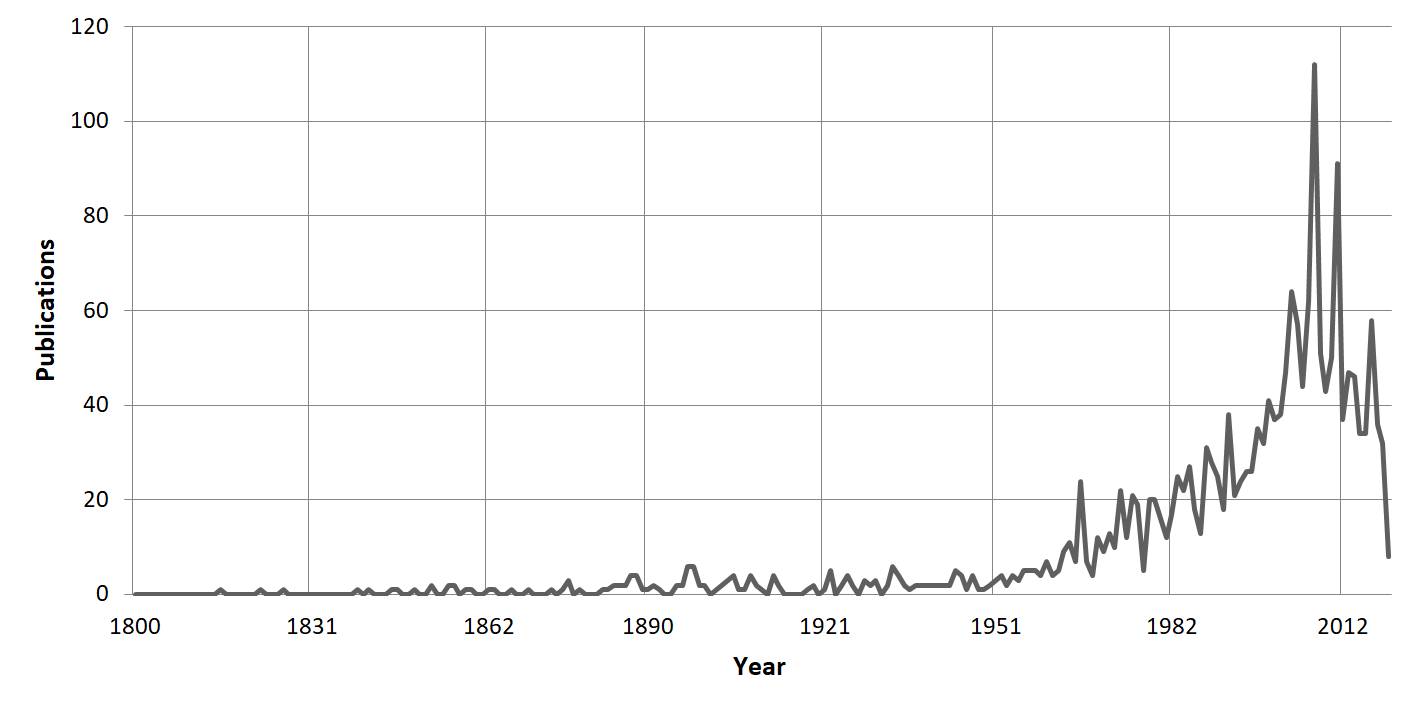
\includegraphics[width=\textwidth]{PublicationsChart.png}
\caption{Number of publications on the \lfam\ family recorded in the Glottolog database by year up to mid 2021 \cite{glottolog}}
\label{fig:PublicationsChart}
\end{figure}


\subsection{Dialects or languages?}\label{s:DialectsorLanguages}
The question of the distinction between a language and a dialect is all-pervasive to linguistics. Different interpretations of this distinction in different research traditions and political systems in the region have created an imbalance in the definition of languages and dialects in the family. \citeA{LaPolla2016} suggests that languages predominantly researched by linguists in the Chinese academic sphere, especially in the Sinitic branch, tend to more commonly be considered dialects of single broader languages, while languages researched by other linguistics, namely in the Indian academic sphere, tend to be considered separate languages in a more closely related subfamily. Anecdotally, I was once told by a Bhutanese person that they believed Bhutan to have 90 different languages, a figure which would require an incredibly fine-grained approach to the definition of languages as opposed to dialects to be true (\citesA{vanDriem1994}{Hyslop2016} suggest a number closer to 20).

This is also reflected at a policy level, namely in how governments identify and classify various ethnolinguistic groups. \citeA{Bradley2002} give an extreme example from the Eastern Indo-Chinese border, where India officially identifies over 50 different ``scheduled tribes'' or ethnic groups, which are all grouped into a single Luoba ``nationality'' across the border by China.

While these two tendencies do not necessarily produce differing results in terms of isolated descriptions (descriptions of separate ``dialects'' of languages spoken in China have been conducted similar to descriptions of separate ``languages'' spoken elsewhere \cites{Lai2017}{TaylorAdams2020}), it can cause skew at a typological level, as there is a possibility that similarly divergent groups of ``languages'' or ``dialects'' will be identified as its own subfamily if spoken in India, but not in China. This has been raised as a potential criticism of \citeA{VanDriem2014} \cite{LaPolla2016}, and presents a potential issue in sampling for this project. That is, will a region of high linguistic diversity be missed or underrepresented because it has been classified in such a way that (deliberately or otherwise) reduces official recognition of this diversity?


\section{Current state of research}\label{s:THOverview:CurrentResearch}
\subsection{State of description}\label{ss:Description:StateOfDescription}
The level of coverage in the description of languages across the \lfam\ subfamilies varies greatly, ranging from subfamilies with over a hundred published grammars, to a number with no published comprehensive grammars, or even no published description at all. In order to compare the state of description across the family and illustrate the disparities, data on language numbers (also presented in Table \ref{t:Methods:SubfamilyLanguageCount}), as well as published literature on each language has been collected from Glottolog \cite{glottolog}. Specifically, the number of unique\footnote{This excluded both exact repetitions in the database where two sources have had the same publication under slightly different names (e.g., with or without middle names or initials), and cases where a two grammars of the same language by the same author are listed, usually because of a thesis which has subsequently been turned into a book. This latter case has been excluded as, while there are likely differences between the two publications, they do not represent the greater level of coverage in the literature that would be seen from a second grammar being written out of an entirely separate project.} publications categorised in Glottolog's database as ``Grammar'' has been counted for each subfamily, as well as the languages of these publications. These figures are estimations, given that the boundary between the distinction in the database between ``Grammar'' and ``Grammar Sketch'' is not a clear line,\footnote{Glottolog does define the categories as ``~150 pages and beyond'' and ``~50 pages'' \cite[Glossary]{glottolog}, though this is not always reflected in practice.} and that the figures rely on Glottolog's very broad but not necessarily perfect coverage of the literature. Similarly, the figures used for the numbers of languages are, of course, also estimations using Glottolog's categorisation. Finally, the database covers publications on grammars dating back at times to the 19th century, which may not be considered up to contemporary standards in terms of linguistic analysis. As such, these figures can certainly be illustrative in a broad sense, showing the differences in documentation levels in general terms, but cannot be seen as precise figures for any further detailed statistical analysis.

The highest coverage was recorded for Meithei, an internal isolate. Glottolog recorded eight unique grammars for the one language, with the earliest being a description by Arthur John Primrose published in 1888\nocite{Primrose1888}. This is by some measure the highest number, with the next highest ratio of languages to grammars seen for the Sinitic subfamily, which has 4.46 grammars for each language.\footnote{116 grammars across 26 languages.} Figure \ref{f:Description:SubfamilyCoverageGraph} shows the ratio of overall grammars per language in each subfamily. Four subfamilies show a ratio of one, meaning there is an equal number of published grammars on the subfamily and languages in the subfamily on Glottolog. This does not mean, however, that every language in the subfamily has been described, as levels of description can vary widely within a given subfamily. While an internal isolate, Meithei serves as a potent example of why this is possible, where multiple grammars have been written on the one language. Similarly, there are cases where the authors of grammars might consider two varieties different languages, or at least sufficiently different for a separate grammar, but the varieties are grouped as one language on Glottolog. For example, of the two English-language grammars on Tshangla (another internal isolate), \citeA{Grollmann2020} discusses specifically the Bjokapakha variety, while \citeA{Andvik2010} covers Tshangla more generally, as external factors prevented him from working with any single given speech community or village. In other cases---for instance \citesA{Gates2021}{Honkasalo2019} writing about Eastern Geshiza and Mazur Stau---it is not necessarily clear whether or not the two rGyalrongic varieties described ought to be considered different languages or not, but are in any case considered grammars of the same language in this analysis and in the source of the data \cite{glottolog}. In this example, \citeA[1]{Honkasalo2019} refers to the specific subgroup within rGyalrongic as the ``Horpa languages,'' while \citeA[12]{Gates2021} uses the same, as well as the more agnostic term ``Horpa lects''.

\begin{figure}
        \centering
        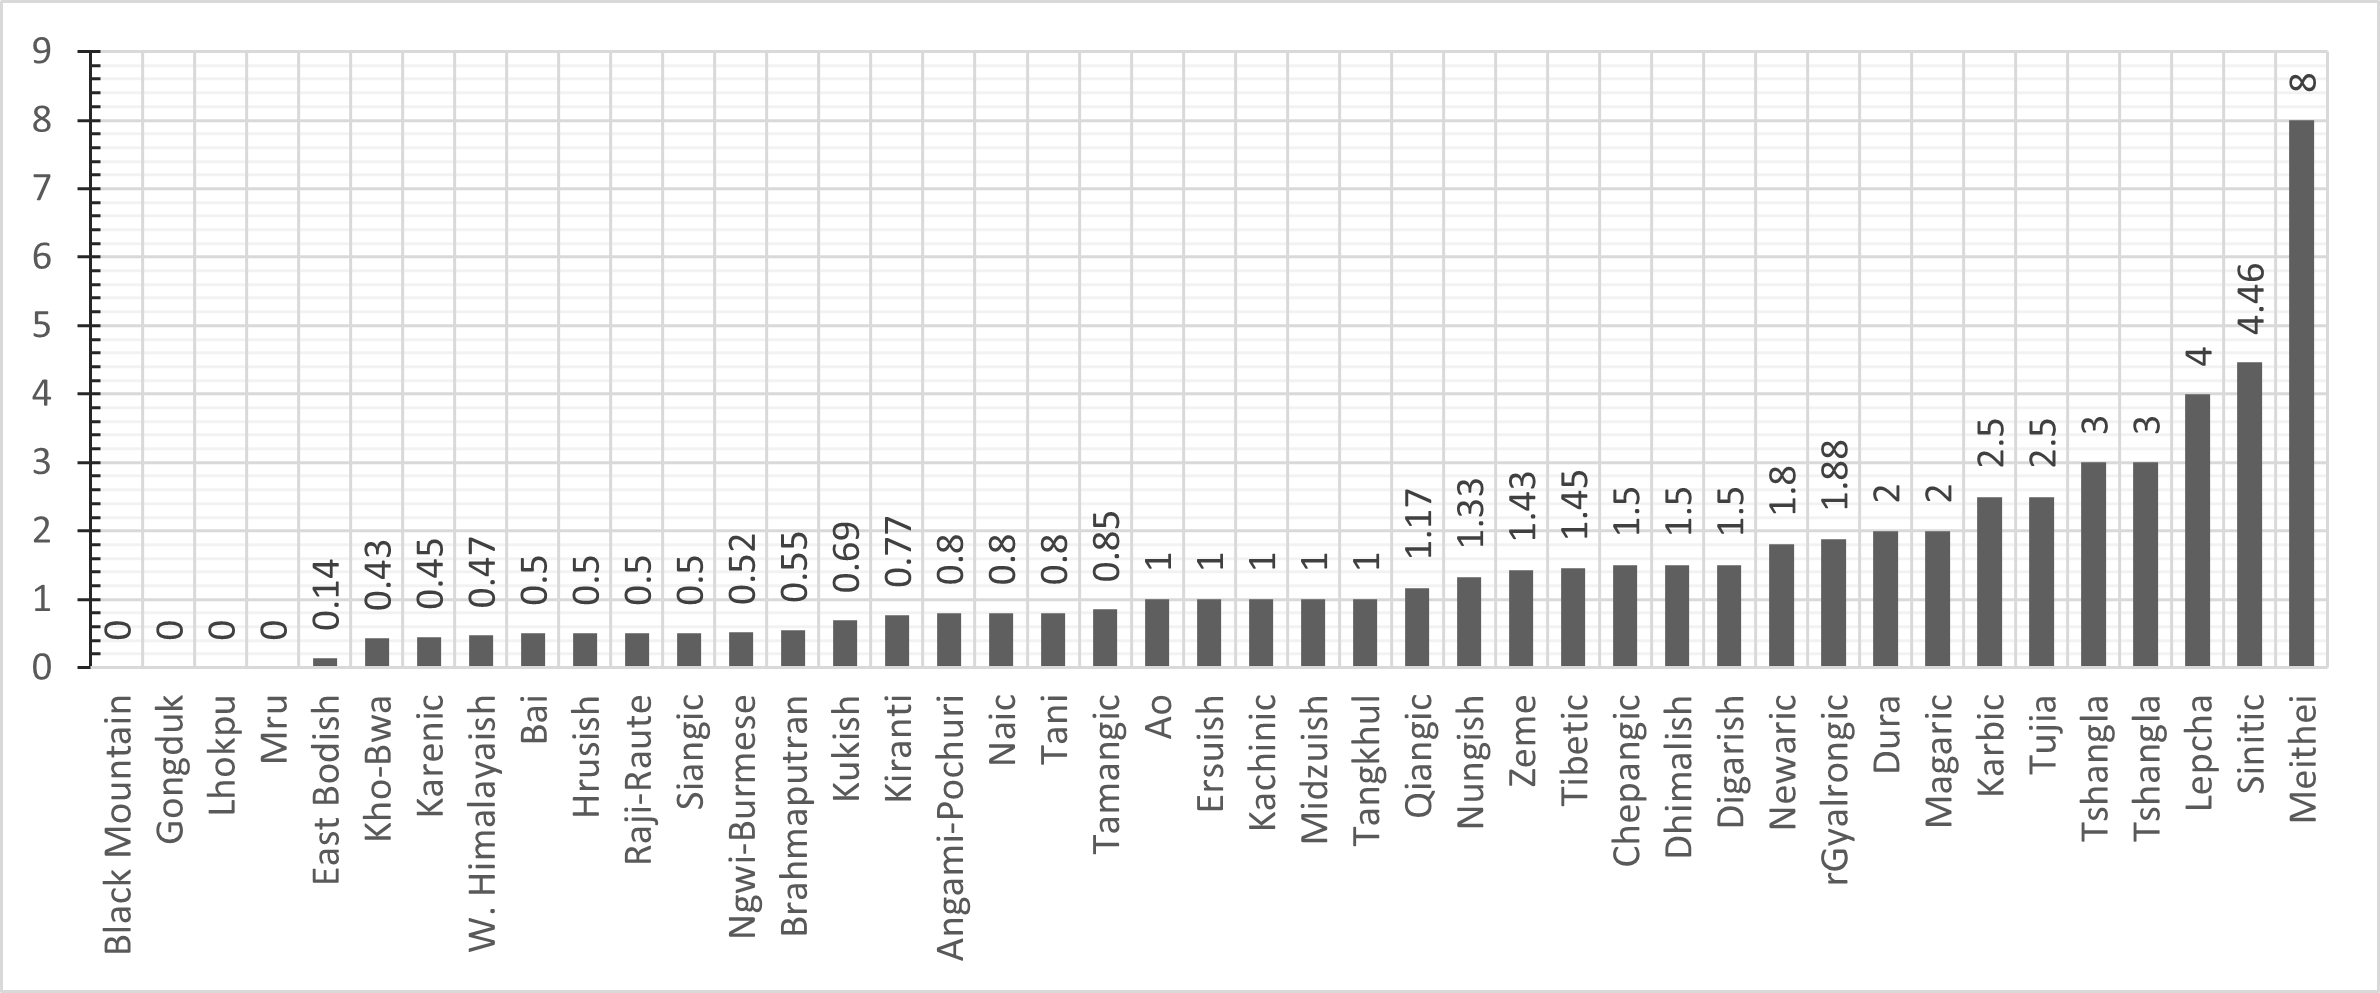
\includegraphics[scale=0.7]{Subfamily Coverage Graph.png}
        \caption{The ratio of overall grammars per language for each of the subfamilies, sorted from lowest to highest.}\label{f:Description:SubfamilyCoverageGraph}
\end{figure}

A comparison of the metalanguages of the literature in this dataset can also reveal some trends; more specifically, it reveals gaps in the data available to this project, given it was limited to literature written in English with some exceptions in texts written in French or German, e.g. \citeA{Lai2017}. This data is presented in Figure \ref{f:Description:SubfamilyCoverageByLanguage}, showing the metalanguages used as a percentage of the total grammars in the dataset. Unsurprisingly, the families with higher levels of literature in Chinese---namely Bai, Digarish, Ersuish, Kho-Bwa, Mizduish, Ngwi-Burmese, Nungish, Qiangic, rGyalrongic, Sinitic, and Tujia---are all at least in part spoken in China. The Digarish, Kho-Bwa, Midzuish, and Nungish branches are all spoken partly outside of China (or in contested areas), specifically in all three cases around the tri-point between China, Myanmar, and the Indian state of Arunachal Pradesh. In these cases as well, the Chinese literature comprises one or two of a total of three or four publications. The higher level of use of French as a metalanguage in the rGyalronic subfamily (4 out of 15) can be attributed directly to the research and teaching of Guillaume Jacques, as three of the items are doctoral theses over which he was supervisor, and the final is his own grammar of Japhug \cite{Jacques2021}.

\begin{figure}
        \centering
        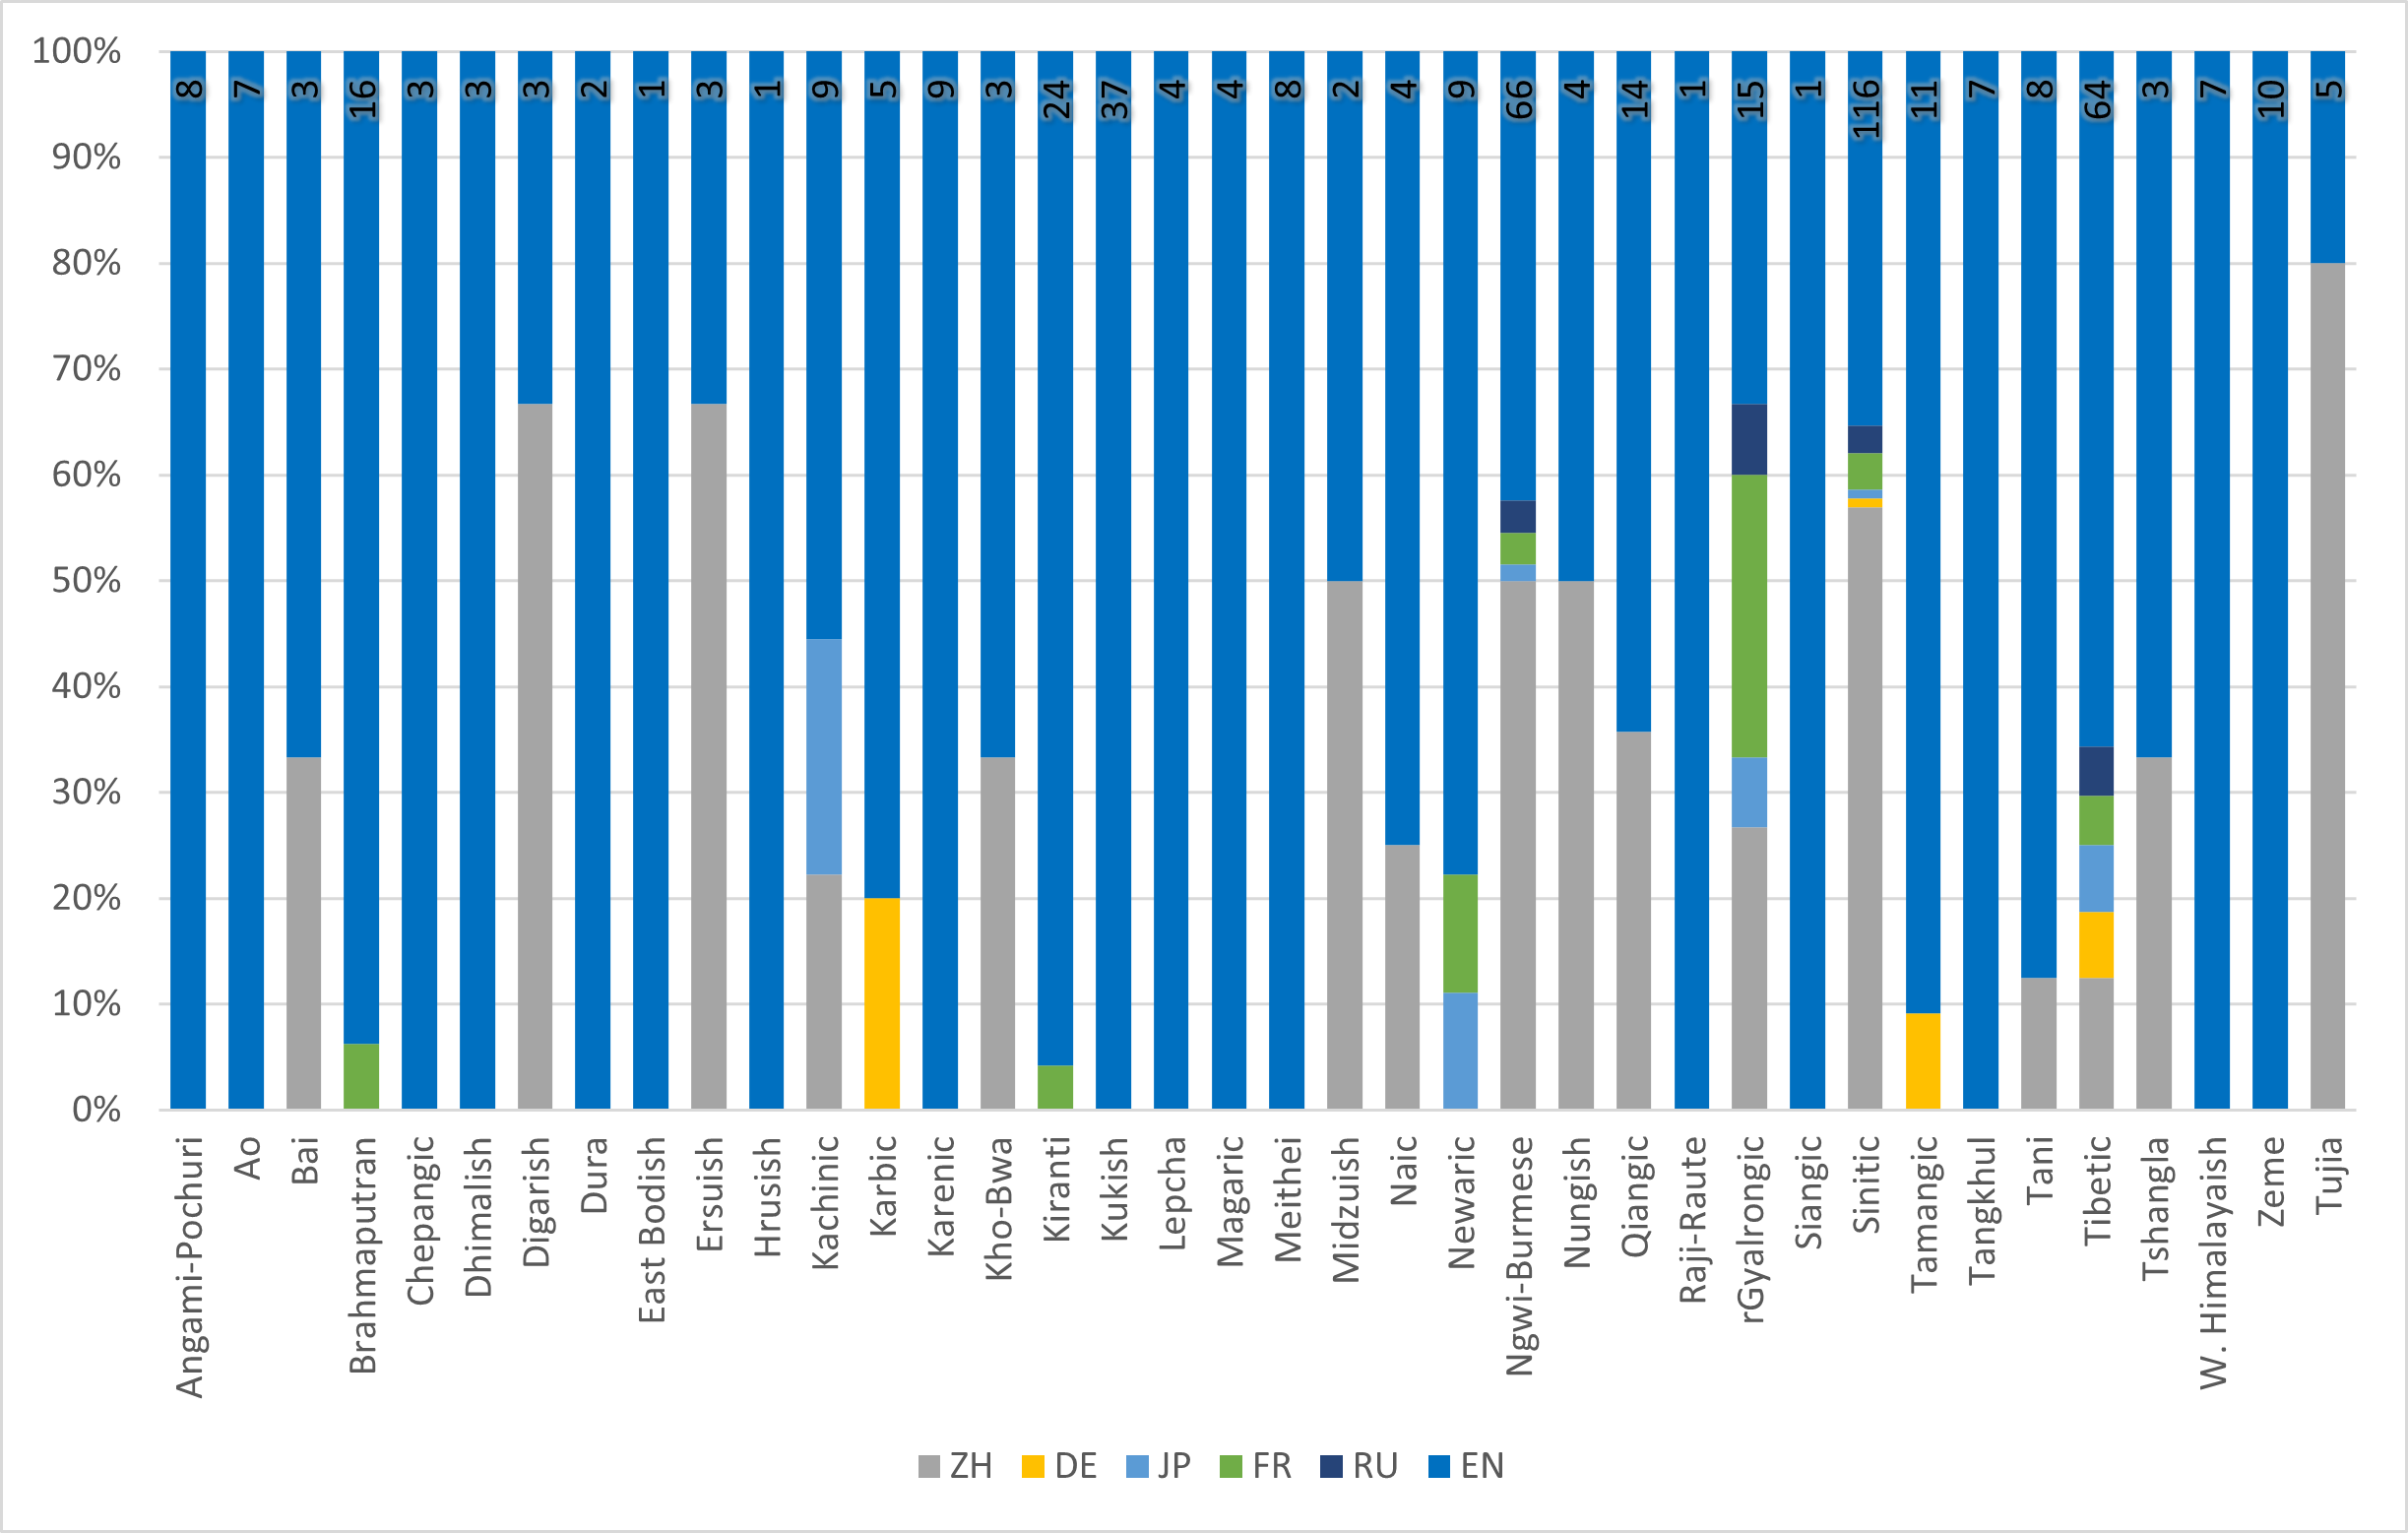
\includegraphics[scale=0.7]{Subfamily Coverage By Language.png}
        \caption{Distribution of metalanguages as a percentage of the total grammars in each subfamily. The number at the top of each subfamily is the total number of grammars in the dataset per sufamily.}\label{f:Description:SubfamilyCoverageByLanguage}
\end{figure}

Thus far, the literature referenced in this analysis has broadly been referred to as ``published'' or as a survey of ``publications''; however it is worth noting that this also includes both Master's and doctoral theses, which have not technically been published or peer-reviewed in the same manner as a book. While this is not to say that a Master's or doctoral thesis is inherently less reliable than a published book, Master's theses in particular are necessarily shorter and less detailed. It was not feasible to annotate all of the grammars in the dataset for their initial origin in these terms, but assuming a higher number of Master's and doctoral students undertaking descriptive projects than degree-holding academics undertaking such projects to the point of a published grammar, it can be assumed that theses comprise a substantial if not majority portion of the dataset.\footnote{While this rings true in the current, I suspect that this has not always been the case. Additionally, the rise of theses being readily available online has made them more accessible, and potentially more common in the Glottolog database.} To compare only the data collected for the larger analysis in this project, discussed in Section \ref{s:Methods:Collection}, about 40\% are Master's or doctoral theses, and theses were generally only used where no formally published book was available.

\subsection{Situating the Sinitic branch in the family}\label{ss:THOverview:HighLevelStructure}

Current opinion on the structure of the family in the literature is strongly divided into two main schools of thought, predominantly centred on the highest-level division in the family genealogically. One school of thought suggests that the family is divided into two primary branches: `Sinitic' and `Tibeto-Burman'. Alternatively, some scholars argue that this binary division is incorrect, and that the Sinitic subfamily exists at a lower level within the overall family. These two mutually exclusive hypotheses will be henceforth referred to as the Sinitic-Divergent and Other-Divergent hypotheses.

A number of recent studies have found evidence in favour of the Sinitic-Divergent hypothesis through computational methodologies \cites{ZhangM2019Baye}{ZhangH2020Baye}{Sagart2019Baye}, namely Bayesian analyses and methodologies from fields of genetics, using cognate sets as an equivalent to genetic markers. While these three papers agree on their support for the Sinitic-Divergent hypothesis to various extents, they otherwise disagree on the internal structure of the Tibeto-Burman branch and the time-scale of the family as a whole. \citeA{Sagart2019Baye} report an origin around 7,400 years BP, with a millet-farming urheimat, in North-Eastern China. \citeA{ZhangM2019Baye} on the other hand reports a slightly younger mean age (about 5,800BP) and an urheimat much further south-west, in the eastern reaches of the Tibetan Plateau. Finally, \citeA{ZhangH2020Baye} suggest an even earlier origin, at 8,000 years BP, and while not providing a clear urheimat, they do suggest that the Sinitic/Tibero-Burman division occurred prior to the development of widespread agriculture in China.

A number of potential issues in these methodologies have been identified by various researchers. \citeA{ZhangH2020Baye} themselves highlight some methodological concerns in \citesA{ZhangM2019Baye}{Sagart2019Baye}, namely surrounding the representativeness of their datasets. They suggest that their dataset presents a more evenly distributed cross-section of the language family by subfamily, with a lower standard deviation in percentage of languages in each subfamily sampled \cite{ZhangH2020Baye}. They also note that \citeA{Sagart2019Baye} contains no data at all from the Karenic or Naga subfamilies, with Karenic languages being spoken geographically much further south than other languages in the family.

This criticism, however, can extend to any study aiming to computationally analyse high level structures of any language family. That is, if a dataset is missing particularly linguistically or geographically divergent data, it is difficult to consider it an accurate representation of the data. Similarly, if data from only one language from a given sub-family is included, but many languages from another, that dataset may be similarly skewed. \citeA{ZhangH2020Baye} notes this as an issue in \citesA{ZhangM2019Baye}{Sagart2019Baye}, and report a more even coverage of each subfamily than in the two previous studies. However, this relies on the subfamilies presented in the paper being representative of the actual subfamilies within the as-yet-unconfirmed \lfam\ stammbaum. There is a degree of a circular logic here. In order to create an even sample of the language family by subfamily, one needs first to know what these subfamilies actually are, which is in many ways exactly what these studies are trying to discover.

\citeA{ZhangH2020Baye} also only report subfamily coverage for a small set of subfamilies, grouping a large number of other languages into the category ``isolates'' and as such ignoring any subfamily relations they may have. In some cases, such as with Tujia or Meithei, this agrees with other literature such as \citeA{VanDriem2014}, though in other cases it seems to fail to consider the language's other close relations. For instance, Kinnauri is listed as an isolate in the list of languages, despite being classified in a separate West Himalayish subfamily by both \citesA{VanDriem2014}{Thurgood2017STIntro}, a subfamily with, in addition to Kinnauri, at least 14 other languages \cite{glottolog}. A similar issue exists with the Kachinic languages, which are represented solely by the so-called `isolate' Jingpo (at the exclusion of 8 other languages), as well as with the rGyalrongic languages, which are represented by Jiarung, Daofu Horpa, and Ergong, all of which are given as isolates despite being grouped together in wider literature \cites{Honkasalo2019}{Gates2021}.\footnote{A pervasive challenge in research on the \lfam\ family is the lack of agreement on language names. `Jiarung' most likely refers to the rGyalrongic languages here, though the core group of the subfamily is varyingly referred to as a group of languages or dialects of a single language. See Section \ref{s:DialectsorLanguages} for further discussion.}

\subsection{Name of the family}\label{ss:THOverview:Name}

This uncertainty surrounding the high level internal structure of the language family also has implications for the name of family itself, in that the historically most widespread name `Sino-Tibetan' specifically references the Sinitic-Divergent hypothesis. A number of alternatives to this have been suggested, either to actively reject the Sinitic-Divergent hypothesis or to remain agnostic. `Tibeto-Burman' has been used fairly widely as an alternative name for the family as a whole, in contrast to Tibeto-Burman as the non-Sinitic branch of a Sinitic-Divergent Sino-Tibetan family \cite{vanDriem2007a}. While this no longer supports a Sinitic-Divergent structure for the family, it also seems to suggest some level of primacy or greater importance to Tibetan and Burmese languages, one of the very issues initially identified with the term Sino-Tibetan. A second alternative, `Trans-Himalayan', has been proposed more recently, avoiding reference to any specific language to avoid any such suggestions of internal structure or greater importance in certain languages or subfamilies \cite{BlenchPost2014}. Here, `Trans-Himalayan' refers to the geographic distribution of languages in the family across entire Himalayan range, and well to the North and South. A potential point of confusion with this name is the inconsistency in meaning between this term and the use of `trans' in wider toponomy. For example, `Transalpine' traditionally refers not to the area across \textit{both} sides of the Alps, but on the \textit{other} side (from Rome), and is contrasted with `Cisalpine' (on \textit{this} side of the Alps).

The term \lfam\ is used in this thesis \lfamreason\

\subsection{Overview of subfamilies}\label{ss:THOverview:Subfamilies}

Van Driem (2014) \nocite{VanDriem2014} presents a large set of subfamilies that are widely agreed on to exist, while avoiding any claims about other internal structures. This phylogenetically agnostic position is referred to as the ``Fallen Leaves'' model, reflecting the confidence with which we can place some languages into various levels of subfamilies (i.e. the leaves) without any claims about their subsequent relationships to each other (i.e. a missing tree structure). This Fallen Leaves model is used throughout this thesis as a foundation for assessing the family as a whole, discussed in detail in \sref{ss:Methods:RepSample}. These subfamilies are illustrated in \figref{fig:SubFamMap}. Subfamily names have been taken directly from \citeA{VanDriem2014}, with the exception of Lolo-Burmese, for which the term Ngwi-Burmese will be used in line with publications such as \citeA{Donlay2019} and \citeA{GonzalezPerez2022}, following \citeA{Bradley2005}.

While \citeA{VanDriem2014} is able to represent well-established subfamilies, uncertainties in the literature arise still in areas with limited description. While there is often a general consensus of which languages are a member of the family and which are isolates or members of other families such as Tai, Austroasiatic, or Indo-European, \citeA{BlenchPost2014} suggest that the lack of research in some areas mean that languages assumed to be \lfam\ simply cannot actually be proven as such (e.g., Hruso, Hrusish: India). They similarly report that some languages in the region are so divergent, it is unclear if they are \lfam\ or languages from a pre-existing family that have undergone heavy \lfam\ influence (e.g., the Siangic subfamily \cite{Post2011}).

\begin{map}

\centering
\includegraphics[width=\textwidth]{SubFamilies.png}
\caption{Approximate geographic distribution of van Driem's (2014) subfamilies. Subfamilies with only one language, or two languages that are not geographically contiguous are represented as single points.}
\label{fig:SubFamMap}
\end{map}

The subfamilies proposed by \citeA{VanDriem2014} can be split into two groups: true subfamilies, and internal isolates. These encompass, respectively, groupings with containing multiple languages as opposed to those containing only one. The ten \lfam\ isolates are as follows:


\begin{itemize}
    \item Black Mountain Mönpa, aka `Olekha, a moribund language spoken in Central Bhutan \cites{vanDriem1995}{Hyslop2016}
    \item Dura, a likely extinct language historically spoken by the Dura people in Lamjung district, Nepal \cite{Schorer2016}
    \item Gongduk, a largely undescribed language spoken in South-Eastern Bhutan spoken by approximately 1000 people in Gongdü Gewog \cite{Bodt2012}.
    \item Lepcha, spoken by 30,000-50,000 speakers in the Indian state of Sikkim and the surrounding regions in Bhutan, Nepal, and the Indian state of West Bengal \cite{Plaisier2007}.
    \item Lhokpu, a largely undescribed language spoken by the Lhop or Doya people in South-Western Bhutan, potentially more closely related to the Dhimalish subfamily \cites{Bodt2012}{Grollmann2018}, discussed in greater detail in \appref{s:Methods:FieldMethods}.
    \item Meithei, aka Manipuri, the primary language of the North-East Indian state of Manipur, where it is spoken by well over 1 million people \cite{Chelliah1997}.
    \item Pyu, an extinct language, historically spoken in modern-day Myanmar prior to the spread of Burmese speakers in the 11th century \cite{Miyake2019}.
    \item Mru, an underdescribed language spoken in the Chittagong Hill Tracts in Bangladesh \cite{VanDriem2014}. It has also been suggested that Mru is closely related to the Anu-Hkongso language spoken on the Bangladesh/Myanmar border \cite{Peterson2017}.
    \item Tshangla, aka Sharchops, spoken by approximately 150,000 people in eastern Bhutan, where it is used as a lingua franca throughout the region. It is also spoken by populations in Arunachal Pradesh, India and in Tibet, where it is called Dirang Monpa and Mòtuō Monpa respectively \cites{Andvik2010}{Grollmann2018}.
    \item Tujia, spoken by approximately 60,000 of the over 8 million members of the Tujia ethnic group in north-western Hunan Province, PRC \cite{Brassett2006}. In Map \ref{fig:SubFamMap} it is divided into Northern and Southern Tujia, the latter of which is estimated to have fewer than 2,000 speakers.
\end{itemize}

The remaining 32 subgroups contain more languages, ranging from two (e.g., Raji-Raute, Siangic, Midzuish) to upwards of 100 (Ngwi-Burmese), and can be seen in \figref{fig:SubFamMap}.

The coverage of literature on the other subfamilies varies substantially between cases. The Tibetic subfamily, for instance, as discussed in Section \ref{s:historyofresearch}, has a long history of grammatical research, as well as a larger population, resulting in greater attention from researchers. As such, there is a significant body of work on Tibetic languages, ranging from full grammars (such as \citesA{Zemp2018}{Graves2007}{Denwood1999}), to extensive discussions about the meanings of single words (see \citesA{Aikhenvald2012Mirative}{DeLancey2012}{Hill2012}{HengeveldOlbertz2012} for one very prominent example).

The Qiangic languages are another subfamily with a comparatively sizable coverage in terms of literature, and most importantly to this project, data availability, with a number of grammars available \cites{LaPolla2003}{Ding2014}, and further research underway.\footnote{Agnes Conrad is working on a descriptive project of Eastern Minyag, a language traditionally classified as Qiangic (p.c. 2024).} According to Glottolog, descriptions are available for at least half of the languages in the subfamily \cite{glottolog}. While many of subfamilies ostensibly have similar levels of coverage, with Glottolog listing between a third to a half as many full grammars as there languages in the subfamily, a number of the smaller non-isolate subfamilies have received little to no attention from descriptive linguists at all. In other subfamilies, specifically those primarily spoken in China or its border regions, descriptions are often more plentiful, but only in Chinese. These include the Ngwi, Midzuish, and of course Sinitic subfamilies, among others, for which only the English (or French in some cases \cite{Lai2017}) literature can be considered in this project. A more in-depth literature review of the state of description in the family can be found in Section \ref{ss:Description:StateOfDescription}.

\subsection{Comparison of proposed phylogenies}\label{ss:Methods:Bayesian}

A substantial contribution to the study of \lfam\ languages, and in particular the historical development of the family in genealogical terms, has been a set of studies using computer statistical modelling, namely Bayesian statistics, borrowed from biology to infer the most likely phylogeny for the family. These studies---\citesA{Sagart2019Baye}{ZhangM2019Baye}{ZhangH2020Baye}---draw varied conclusions about the internal structure of the family and the timeline of its development, though all draw the conclusion that the Sinitic subfamily is most likely either the sole outgroup, or, per \citeA{ZhangH2020Baye}, one of two.

Given their disagreement, and the discussion thus far about their methodology, this section will compare the phylogenies provided in \citesA{Sagart2019Baye}{ZhangM2019Baye}{ZhangH2020Baye}, as well as comparing all three to the Fallen Leaves model \cite{VanDriem2014}. Some other proposed phylogenies, such as that put forward in \citeA{STEDT}, are not included here as they remain largely agnostic about the family's structure outside of a few primary divisions. In Figures \ref{f:Methods:Sagart}-\ref{f:Methods:Zhang2020}, the trees given in their respective sources are reproduced to the subfamily level. That is, the branches are reproduced exactly, but rather than terminating in individual languages (as in \citesA{Sagart2019Baye}{ZhangM2019Baye}{ZhangH2020Baye}), or in other subfamilies, the branches terminate in the equivalent subfamily from the set used in this project given in Table \ref{t:Methods:SubfamilyLanguageCount}. While the branching structure of the subfamilies is accurately reproduced here, the time depth of the various divergences given in the Bayesian analyses is not.

Not every subfamily is represented in every tree, a point which forms part of the criticism of the Bayesian analyses. This occurs for these analyses when a given sample does not include any data from a given subfamily, and therefore does not represent or account for it in the final result. Missing subfamilies for each of \citesA{Sagart2019Baye}{ZhangM2019Baye}{ZhangH2020Baye} are given in Table \ref{t:Methods:BayesMissingSubfamilies}.

\begin{sidewaysfigure}
\centering
  \scalebox{0.5}{\begin{forest} 
   phylogeny,
[\lfam 
[
  [,tikz={\node [draw,red,fit to=tree] {};}
    [Kachinic]
    [Brahmaputran]
  ]
  [Sinitic,tikz={\node [draw,red,fit to=tree] {};}]
]
[
  [
    [Karbi]
    [,tikz={\node [draw,red,fit to=tree] {};}
      [Tangkhul]
      [Kukish]
    ]
  ]
  [
    [
      [Chepang]
      [
        [Tshangla]
        [,tikz={\node [draw,red,fit to=tree] {};}
          [Tani]
          [Digarish]
        ]
      ]
      [Kiranti,tikz={\node [draw,red,fit to=tree] {};}]
    ]
    [
      [W. Himalayish,tikz={\node [draw,red,fit to=tree] {};}]
      [
        [Nungish]
        [,tikz={\node [draw,red,fit to=tree] {};}
          [Tibetic]
          [
            [
              [Qiangic]
              [rGyalrongic]
            ]
            [Ngwi-Burmese]
          ]
        ]
      ]
    ]
  ]
]
]
\end{forest}}
\caption{The \lfam\ family as per \citeA{Sagart2019Baye}, showing the positions of the subfamilies used in this project. Branches with over 80\% posterior probability (that is, branches with high confidence) have been marked with a red box. Time depth has not been reproduced in this tree.}
\label{f:Methods:Sagart}
\end{sidewaysfigure}

\begin{sidewaysfigure}
  \centering
  
    \scalebox{0.45}{\begin{forest} 
    phylogeny,
  [\lfam 
      [Sinitic,tikz={\node [draw,red,fit to=tree] {};}]
      [
          [
            [Karen]
            [,tikz={\node [draw,red,fit to=tree] {};}
              [Kukish]
              [
                [Ao]
                [
                  [
                    [Tangkhul]
                    [Zeme]
                  ]
                  [Angami-Pochuri]
                ]
              ]
            ]
          ]
          [
            [,tikz={\node [draw,red,fit to=tree] {};}
              [Kachinic]
              [Brahmaputran]
            ]
            [
              [
                [Digarish]
                [Tani]
              ]
              [
                [
                  [
                    [Kiranti]
                    [,tikz={\node [draw,red,fit to=tree] {};}
                      [Chepang]
                      [Magar]
                    ]
                  ]
                  [Nungish,tikz={\node [draw,red,fit to=tree] {};}]
                ]
                [
                  [West Himalayish]
                  [
                    [,tikz={\node [draw,red,fit to=tree] {};}
                      [Tamangic]
                      [
                        [Tibetic]
                        [East Bodish]
                      ]
                    ]
                    [,tikz={\node [draw,red,fit to=tree] {};}
                      [
                        [Nàic]
                        [
                          [Ersuish]
                          [
                            [Qiangic*]
                            [rGyalrongic*]
                          ]
                        ]
                      ]
                      [Ngwi-Burmese]
                    ]
                  ]
                ]
              ]
            ]
          ]
      ]
  ]
  \end{forest}}
  \caption{The \lfam\ family as per \citeA{ZhangM2019Baye}. *The phylogeny here does not in fact support these two subfamilies, but rather gives two rGyalrongic languages -- rGyalrong Maerkang (glottolog: Situ) and Caodeng (glottolog: Tshobdun) -- as an outgroup to the Qiangic clade, and two others -- Daofu and Ergong Danba (glottolog: both under Stau-dGebshes) are given as members of one of two Qiangic branches. Branches with over 80\% posterior probability have been marked with a red box. Time depth has not been reproduced in this tree.}\label{f:Methods:Zhang2019}
  \end{sidewaysfigure}

  \begin{sidewaysfigure}
    \centering
    
      \scalebox{0.35}{\begin{forest} 
phylogeny,
    [\lfam 
      [
        [Sinitic,tikz={\node [draw,red,fit to=tree] {};}]
        [
          [,tikz={\node [draw,red,fit to=tree] {};}
            [Lepcha]
            [Kiranti]
          ]
          [
            [
              [W. Himalayish]
              [
                [Digarish,tikz={\node [draw,red,fit to=tree] {};}]
                [,tikz={\node [draw,red,fit to=tree] {};}
                  [Siangic]
                  [Tani]
                ]
              ]
            ]
            [
              [,tikz={\node [draw,red,fit to=tree] {};}
                [Kachinic]
                [Brahmaputran]
              ]
              [
                [Kho-Bwa,tikz={\node [draw,red,fit to=tree] {};}]
                [Hrusish,tikz={\node [draw,red,fit to=tree] {};}]
              ]
            ]
            [
              [
                [
                  [
                    [Magaric*]
                    [Karen,tikz={\node [draw,red,fit to=tree] {};}]
                  ]
                  [
                    [Dhimalish]
                    [
                      [Magaric*]
                      [Chepangic]
                    ]
                  ]
                ]
                [
                  [Karbi]
                  [
                    [Kukish,tikz={\node [draw,red,fit to=tree] {};}]
                    [
                      [Meithei]
                      [,tikz={\node [draw,red,fit to=tree] {};}
                        [
                          [Angami-Pochuri**]
                          [Ao]
                        ]
                        [
                          [Tangkhul]
                          [
                            [Zeme]
                            [Angami-Pochuri**]
                          ]
                        ]
                      ]
                    ]
                  ]
                ]
              ]
              [
                [
                  [Midzuish]
                  [Nungish,tikz={\node [draw,red,fit to=tree] {};}]
                ]
                [
                  [
                    [Tamangic,tikz={\node [draw,red,fit to=tree] {};}]
                    [
                      [Tshangla]
                      [,tikz={\node [draw,red,fit to=tree] {};}
                        [East Bodish]
                        [Tibetic]
                      ]
                    ]
                  ]
                  [
                    [Tujia]
                    [
                      [
                        [rGyalrongic***]
                        [,tikz={\node [draw,red,fit to=tree] {};}
                          [
                            [Ngwi-Burmese†]
                            [Ersuish]
                          ]
                          [
                            [Qiangic]
                            [rGyalrongic***]
                          ]
                        ]
                      ]
                      [Ngwi-Burmese,tikz={\node [draw,red,fit to=tree] {};}]
                    ]
                  ]
                ]
              ]
            ]
          ]
        ]
      ]
    ]
    \end{forest}}
    \caption{The \lfam\ family as per \citeA{ZhangH2020Baye}. In this analysis, a number of van Driem's (2014) subfamilies are divided, with either single or multiple languages separated from the rest of their subfamily. These have been marked (*, **, ***, †) and are discussed in the text. Branches with over 80\% posterior probability have been marked with a red box. Time depth has not been reproduced in this tree.}\label{f:Methods:Zhang2020}
    \end{sidewaysfigure}

As discussed above, for each of the terminal nodes given in Figures \ref{f:Methods:Sagart}-\ref{f:Methods:Zhang2020} (that is, van Driem's Fallen Leaves), one to three languages have been sampled. While initially the intention of presenting Figures \ref{f:Methods:Sagart}-\ref{f:Methods:Zhang2020} was to compare the representativeness of this project's sample against their proposals for a phylogeny of the \lfam\ family, it is clear from \tabref{t:Methods:BayesMissingSubfamilies} that, in all cases, the coverage of this project is substantially larger, especially in terms of smaller language families or internal isolates. As \citeA{VanDriem2014} categorised the entire family into generally very fine-grained subfamilies, there are no languages in any of the three studies that cannot be categorised into one of the subfamilies used in this project, implying a lack of gaps in this project's sample. As such, to identify possible gaps in this survery's sample, it is necessary to identify locations where \citesA{Sagart2019Baye}{ZhangM2019Baye}{ZhangH2020Baye} disagree with \citeA{VanDriem2014}. A number of small disagreements are noted for \citesA{ZhangM2019Baye}{ZhangH2020Baye}

Another significant area of consideration is instances wherein van Driem's (2014) larger subgroups are presented as multiple smaller subfamilies in the other data. Namely, \citeA{ZhangM2019Baye} divides the Ngwi-Burmese family into three classifications, diverging approximately 2,000 years ago. Taking these three branches (Loloish, Nusu, Burmish) as separate subfamilies for the sake of representativeness, the sample for this project thus contains two Loloish (here: Ngwi) languages, one Burmish language, and no Nusu languages. As is discussed above, the Ngwi-Burmese subfamily is the largest by some margin, which gives some credence to a division into multiple smaller subfamilies. However, when considering the estimated age of the subfamily per the Bayesian analyses, the combined Ngwi-Burmese branch is a similar age to many of van Driem's (2014) other subfamilies represented in \citeA{ZhangM2019Baye}---which range from ~750 years old for Tani to ~3,000 years old for Kiranti---as well as in \citeA{ZhangH2020Baye}, in which the subfamilies vary in age from ~500 years old (Ersuish) to ~4,500 years old (West Himalayish). This is to say that although there are a great number of contemporary Ngwi-Burmese languages attested, the branch itself does not appear to be any older than many of the smaller branches used in this survey, and as such there is less of a reason to treat it as too large or too high-level.



\begin{table}\caption{Subfamilies not represented in the initial data or results of \citesA{Sagart2019Baye}{ZhangM2019Baye}{ZhangH2020Baye}. Internal isolates are given in italics. * Bai was specifically excluded in this study as the extensive borrowing from Sinitic languages would cause problems for the analysis.}\label{t:Methods:BayesMissingSubfamilies}
  \centering
  \begin{tabular}{l | l | l}
    \hline
    \citeA{Sagart2019Baye} & \citeA{ZhangM2019Baye} & \citeA{ZhangH2020Baye} \\
    \hline
    Angami-Pochuri & Bai & Bai* \\
Ao & Black Mountain & Black Mountain \\
Bai & Dimalish & Dura \\
Black Mountain & Dura & Gongduk \\
Dimalish & Gongduk & Lhokpu \\
Dura & Hrusish & Mru \\
East Bodish & Karbi & Naic \\
Ersuish & Kho-Bwa & Newaric \\
Gongduk & Lepcha & Pyu \\
Hrusish & Lhokpu & Raji-Raute \\
Karenic & Meithei &  \\
Kho-Bwa & Midzuish &  \\
Kukish & Mru &  \\
Lepcha & Newaric &  \\
Lhokpu & Pyu &  \\
Magaric & Raji-Raute &  \\
Meithei & Siangic &  \\
Midzuish & Tshangla &  \\
Mru & Tujia &  \\
Naic &  &  \\
Newaric &  &  \\
Pyu &  &  \\
Raji-Raute &  &  \\
Siangic &  &  \\
Tamangic &  &  \\
Tujia &  &  \\
Zeme &  &
  \end{tabular}
  
\end{table}

The unrepresented subfamilies shown in Table \ref{t:Methods:BayesMissingSubfamilies} are, to an extent, a good indicator for how representative the given samples are. Of course, some of the missing data is unavoidable, and is repeated in this project, namely for Raji-Raute, Gongduk, Black Mountain, and Pyu. \citeA{ZhangH2020Baye} specifically report that Bai (marked with an asterisk in Table \ref{t:Methods:BayesMissingSubfamilies}) was excluded due to its high level of borrowing from Sinitic languages, which causes problems when comparing cognates. For \citeA{ZhangH2020Baye}, this leaves only a few smaller subfamilies unrepresented, and for \citeA{ZhangM2019Baye} a few more, though most are still fairly small or underdocumented. \citeA{Sagart2019Baye}, however, has a few more glaring omissions, in addition to the smaller or inaccessible subfamilies excluded by the others. Namely, no data from any Karenic, Kukish languages were included, nor from the smaller and (at least according to \citesA{ZhangM2019Baye}{ZhangH2020Baye}) closely related Angami-Pochuri and Ao subfamilies. As has been already pointed out in \citeA{Hyslop2020Millet} and even in \citeA{ZhangH2020Baye}, these omissions are problematic in a quantitative analysis in which a representative sample is indispensible, especially given the much wider coverage of \citeA{ZhangH2020Baye} compared to the two earlier studies. Even in cases where data are simply not available, the large gaps in documentary research across the \lfam\ family may mean that, at this stage, the sort of quantitative statistical research undertaken in these projects is simply not yet viable, at least until a truly representative sample can be developed. Such a sample would not necessarily include data from all of the currently underdescribed languages, but it would at least be informed by a better understanding of relationships between families. For instance, if further evidence proves further that Lhokpu can be grouped into a Dimalish subfamily with Dhimal and Toto, then it need not be included separately if that family is already sufficiently represented. Similarly, further research on the other underdescribed languages of Bhutan, Gongduk and Black Mountain Mönpa, may well allow them to quite clearly be aligned with existing subgroups, but may also distance them further from any clear classification, further necessitating their inclusion in a representative sample of the family.

There is the potential here for a certain circular logic in developing a sample to be used for research into phylogenies, in that the development of a representative sample must be informed by a general understanding of the phylogeny of the family in order to sufficiently and more or less equally survey all areas of the family. This understanding, however, is exactly the outcome the research itself is attempting to attain. This is further confounded by the uncertainty these studies have regarding any reconstructions to deeper time depths, as is discussed below.

Only briefly discussed in \citeA{ZhangH2020Baye} is the statistical confidence surrounding the various bifurcations given in the study's proposed phylogeny. While the study does not suggest that the given tree is clearly correct, it does suggest that the results of the analysis could be used to inform further studies into the history of the people of the Himalayas \cite[5]{ZhangH2020Baye}. The posterior probability of a given divergence is the calculated likelihood of the given branch being valid given the input data and starting parameters ranging from 0 (no  confidence) to 1 (complete confidence) \cite{Alfaro2006}. It can be seen as the probability that everything under a given branch belongs under that branch at the exclusion of others. For instance, the root of the tree will always have a posterior probability of 1, as the entire tree falls under it and there are no alternatives. While in biology, strongly supported clades need a posterior probability of 0.95, no such consensus has been reached in linguistics, with given thresholds for valid trees ranging from 0.7, 0.9, or with no threshold at all \cite{Dolin2022}. The middle level divergences in \citeA{ZhangH2020Baye} fall well below these thresholds, with the lowest falling as far as 0.04 (or 4\% confidence) in certain places. In one case, a proposed bifurcation is estimated to have occurred earlier than that of its proposed parent, which is not possible. The result of this is that for most divergences proposed to have occurred earlier that 4,000 years before present, there is little to no confidence from the analysis that the final output is correct. \citeA{ZhangH2020Baye} do note that they have over a posterior probability of over 0.95 for a number of clades at various levels. Although there are a number of clades and subfamilies it does confidently claim, for the most part it cannot actually make any confident claims about the relationships of these lower level clades to each other.\footnote{I discuss this in depth here as, while these figures are clearly presented in \citesA{Sagart2019Baye}{ZhangH2020Baye} and in the supplementary materials for \citeA{ZhangM2019Baye}, I do not believe the actual meaning of these figures would be particularly accessible to a linguist who did not otherwise specialise in this area. The results are provided faithfully and the well-supported clades are listed by \citeA[3]{ZhangH2020Baye}, but the extent to which many of the other clades are \textit{not} supported, and as such the extent to which the analyses do not particularly draw conclusions beyond what is possible with traditional methods, is not, I believe, made clear enough that a linguist working on \lfam\ languages would, on first read, understand the conclusions actually being drawn.} An exception to this is for the Sinitic languages, which were placed as an outgroup with a posterior probability of 0.8. Clades with posterior probabilities of over 0.8 (80\% confidence) have been highlighted on the figures above in red boxes, and can be seen as the clades about which the analysis is able to make a claim over. That is, in Figure \ref{f:Methods:Zhang2020} for example, there is sufficiently strong evidence to support the Kukish subfamily, as well as a clade of the Angami-Pochuri, Ao, Tangkhul, and Zeme subfamilies, but the branches connecting them do not have sufficiently strong evidence to view them as a valid claim.

\citeA{ZhangM2019Baye} overall do not reach the same low posterior probabilities as in \citeA{ZhangH2020Baye}, though they do still only report higher probabilities at smaller subfamily levels, with probabilities below 0.5 (50\%) for many of the high level divergences. This suggests that, while more confident than the other analysis, it is still unable to make any solid claims regarding the relationships of well-established clades to one another. \citeA{Sagart2019Baye} explicitly use a cutoff of 0.8 for their confident clades, and face a similarly uncertain high-level phylogeny. They do, however, report high confidence for a large clade including Tibetic, Qiangic, rGyalrongic, and Ngwi-Burmese languages they label ``Tibeto-Dulong'' (p. 10318) to a time depth of approximately 5,000 years before present. \citeA{ZhangH2020Baye} report a posterior probability of 0.33 for this grouping.

With this noted, van Driem's (2014) uncertainty surrounding relationships between established subfamilies remains to an extent in these studies. Some relationships with a shallower time depth are reported (though inconsistently between analyses) to a larger scale than in the model used for this project, but at the highest level the relationships between different branches of the family remain unclear for both the more traditional comparative method and the more recent Bayesian analysis. This further supports the decision here to approach the development of a representative sample from a phylogenetically agnostic foundation.


\section{Historical linguistics}
\subsection{Ancient literary languages}\label{s:AncientLiteraryLanguages}
The disagreement in the field surrounding the overall phylogeny of the family was discussed in Section \ref{ss:THOverview:HighLevelStructure}, but this only addressed research on the family at a higher level, and using the computational models. The question remains of what research has been conducted at a lower level, and what reconstructions have been thus far possible.

While not common throughout the \lfam-speaking sphere, there are a number of sources of early written language that have been used in historical linguistics in the region. As discussed in Section \ref{s:historyofresearch}, primary historical sources are available in both Old and Middle Chinese and Old and Classical Tibetan. In addition to these, bodies of writing exist in the Pyu language of modern day Myanmar, as well as Old Burmese, and the Tangut language of north-western China.

The Pyu language was likely spoken throughout the First Millennium  by the pre-Bamar population of modern-day Myanmar. The language survives in early Buddhist inscriptions, and has only recently been decoded in earnest by linguists \cites{Griffiths2017}{Miyake2019}. Pyu seems to have largely been replaced by Old Burmese from the 11th century CE following the migration of the Bamar people into the Irrawaddy Valley and advent of the Bagan Kingdom \cites{Wheatley2017}{Griffiths2017}. Old Burmese is the direct parent of Modern Burmese, and also largely survives in Buddhist inscriptions.

Tangut was spoken in the North-Western Chinese empire of Xixia in the early second millenium \cite{Gong2017}. It may be an early member of the Qiangic subfamily, though not an ancestor of any modern Qiangic languages \cite{Matisoff2004}. However, more recent research suggests instead that the language may be closer to the Western rGyalrongic group \cite{Lai2020}, with some shared forms discussed in Section \ref{ss:Discussion:EasternGeshiza}. The language was lost until the early 20th century, when a body of literature was discovered in the ruins of the Tangut city of Khara Khoto \cite{Gong2017}. Descriptive and analytical work is ongoing.

The Nam language is another language of the region known only through historical writings, but it has not yet been deciphered \cite{Ikeda2012}.

Aside from these few surviving records, and for the most part their descendants (that is, Modern Burmese, the Tibetic languages, Sinitic Languages, as well as the Yi languages in Southern China), there are little to no historical written traditions throughout the \lfam-speaking world, a characteristic which is shared with much of upland south-east Asia. A number of other languages do have native writing systems, some of which can be dated to a remarkable time depth. The oldest record of the Meithei writing system is a copper plate dating to the 8th century CE, though most of the surviving records are much younger, from the 16th-17th centuries \cite{Chelliah2000}. Other languages with native writing systems with long histories of use, and subsequently a native literary tradition and historical linguistic record, include Lepcha and Limbu. Both writing systems appear to have been developed by Buddhists around the early 18th century \cite{Plaisier2007}, though little historically oriented work has been published to the best of my knowledge. On the other hand, some native scripts are much more recent inventions. The Pollard and Fraser scripts, both used to write Lisu (Ngwi-Burmese) and some surrounding languages, were developed by missionaries for the purposes of Bible translation in the early 20th century \cite{Bradley2017}. Community developed scripts for Wancho (Brahmaputran), Tangsa (Brahmaputran), Toto (Dhimalish), and Kayah Li (Karenic), developed across the last 50 years, have also been added to Unicode. However, given their recent development, these do not add anything to the historical study of \lfam\ languages.

One potential factor in the general lack of written language compared to surrounding areas is investigated by \citeA{Scott2009} in his anthropological survey of the similarities and shared histories of groups in the south-east Asian Massif, referred to as \textit{Zomia}. In this analysis, he identifies the active rejection of and departure from state control as a uniting factor throughout the region, and addresses the cultural similarities that could stem from this common history.

Despite focussing primarily on the south-east Asian uplands, Scott's (2009) analysis of Zomia as a cultural region united by a rejection of the powerful states in the region and a subsequent retreat into highland areas, can be used as a frame to view the \lfam-speaking groups throughout much of the Himalayas. Namely, Scott reports a tradition of oral history and a rejection of written literary tradition throughout Zomia, a situation largely mirrored throughout the Himalayas, where few languages and subfamilies have any traditional written tradition. The reasons for this avoidance of written language in Zomia seem to also hold in the Himalayas, in that written language can be considered representative of state control (see \citeA[229]{Scott2009} for specific examples in south-east Asia). A similar distrust of writing, especially contracts, can be seen today in the Himalayas. \citeA{VanDriem2016} refers to anecdotes of language informants in Bhutan being fearful of signing contracts as part of a researcher's formal ethics process, and to request the use of such formalised and state-governed written language was seen as, at the very least, rude.  As such, it is perhaps not enormously surprising that much of the \lfam-speaking upland regions do not have any surviving literary tradition, or historical linguistic research as with the above, which can be drawn upon by contemporary linguistics.
%\todo{I might remove this whole section honestly, not sure if it's really worth saying - or if it's even that valid}

The paucity of historical written traditions in the \lfam\ family, especially when compared to the substantial diversity and divergence in all branches of the family, has meant that, while these historical languages have provided indispensable data for research into their descendants (e.g., into the development of forms in the various modern Tibetic languages), they have not provided a central foundation for reconstruction of any \lfam\ proto language \cite{STEDT} (in contrast with the importance of Latin, Ancient Greek, Sankrit, etc. in Indo-European linguistics, for instance).

\subsection{Reconstruction work}
Reconstruction of \lfam\ languages has been attempted for much of the history of Western research on the family. A major early piece of work in this tradition is \citeA{Benedict1972}, originally written in the early 1940s following the depression-era project \textit{Sino-Tibetan Lingusitics} led by Robert Shafer, and remaining unpublished for some 30 years. The eventual 1972 publication features revisions and annotations by James Matisoff, including extra data from Matisoff's own research and other more recent findings. \citeA{Matisoff2003} reports that while many reconstructions have since been revised in light of new data, the cognate sets collected and collated by Benedict remain valid. Even more recent reconstructions, such as the aforementioned \citeA{Matisoff2003} (which attempts to reconstruct just the non-Sinitic branches of the family as per the Sinitic-divergent theory discussed in Section \ref{ss:THOverview:HighLevelStructure}), have seen significant controversy, evident in the dialogue starting with Sagart's (2006) \nocite{Sagart2006} review of \citeA{Matisoff2003}, and continuing to Matisoff's (2007) \nocite{Matisoff2007} response and Sagart's (2008) \nocite{Sagart2008} subsequent reply. This handbook was the first major publication in the Sino-Tibetan Etymological Dictionary and Thesaurus (STEDT) project, running from 1987 to 2015, which has produced a sizeable dictionary of nearly 6,000 reconstructions to a Proto-Sino-Tibetan \cite{STEDT}.

In addition to this work at the family level, research has been undertaken to reconstruct the common ancestors for the numerous subfamilies. These include reconstructions of the Tani family \cite{Sun1993}, Kukish languages \cite{VanBik2009}, East Bodish languages \cite{Hyslop2014a}, and many others, often themselves products of the STEDT project (such as \citesA{Button2011}{Bruhn2014} in addition to those cited above).

\section{Summary}
While research on individual \lfam\ languages, in particular those of states and religions, has a long history, widespread documentation of languages, in particular of endangered or minority languages, remains in its infancy. With this paucity of descriptive research across the very large family, a bigger picture view of the family as a whole in terms of its development remains unavailable. Despite various phylogenies being proposed by a number of studies discussed in \sref{ss:Methods:Bayesian}, none have thus far been able to draw any stronger conclusions than have been drawn using the traditional comparative method, being a series of variously well established local subfamilies or unclear or unproven relation to each other beyond their position as \lfam\ languages. The \lfam\ family represents a useful platform for a broad typological survey such as this one, in that it is large and hugely varied, evidenced by the lasting uncertainty about the historical development of the family. However, is still constrained by its nature as a primary language family, as every language is, to the best of our knowledge, ultimately related to every other.